\subsection{Structure of Storage Media}\label{subsec:Structure_Storage_Media}
In this section, the structure of secondary storage is discussed.
Starting with the physical structure of magnetic disks, magnetic tapes, and solid-state storage.

\subsubsection{Magnetic Disks}\label{subsubsec:Magnetic_Disks}
Magnetic disks (typically called hard drives) provide the bulk of storage.
Inside each unit, there are disk platters that have a flat circular shape.
The two surfaces of a platter are covered with a magnetic material.
Information is stored by recording it magnetically on the platters.
Typical disks can transfer several megabytes of data per second, and they have seek times and rotational latencies of several milliseconds.

\begin{itemize}[noitemsep]
\item A read–write head ``flies'' just above each surface of every platter.
\item The heads are attached to a disk arm that moves all the heads as a unit.
\item The surface of a platter is logically divided into circular tracks, which are subdivided into sectors.
\item The set of tracks that are at one arm position makes up a cylinder.
\end{itemize}

\begin{figure}[h!tbp]
  \centering
  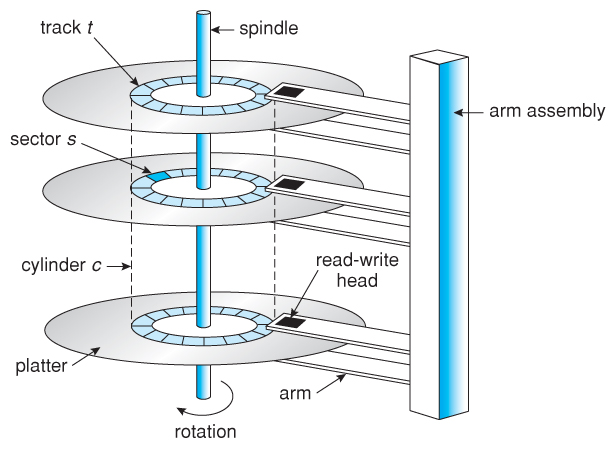
\includegraphics[scale=0.8]{./Drawings/EDAF35-Operating_Systems/Magnetic_Disk_Mechanism.jpg}
  \caption{Magnetic Disk Moving head Mechanism}
  \label{fig:HDD_Mechanism}
\end{figure}


%%% Local Variables:
%%% mode: latex
%%% TeX-master: "../../EDAF35-Operating_Systems-Reference_Sheet"
%%% End:
